% Configuración a 2 columnas

\documentclass[3p]{elsarticle}
%\documentclass[3p,twocolumn]{elsarticle}

% Paquete con el tipo de codificación del lenguaje
\usepackage[utf8]{inputenc}
% Paquete para mostrar el número de líneas
\usepackage[modulo]{lineno}
\linenumbers
% Paquete para mostrar imágenes
\usepackage{graphicx}
\graphicspath{ {/home/acamon/TFG/GitHub/TFG/Recursos/Fotos/} }
% Paquete para resaltar enlaces y referencias
\usepackage{hyperref}
% Configuración del paquete
\hypersetup{
  breaklinks=true,  
  colorlinks=true,
  urlcolor=urlcolor,
  linkcolor=linkcolor,
  citecolor=citecolor,
}

% Modifica el formato de las referencias
\biboptions{sort&compress}

% Modifica el pie de la primera página para poner el número de la misma
\makeatletter
\def\ps@pprintTitle{%
   \let\@oddhead\@empty
   \let\@evenhead\@empty
   \def\@oddfoot{\reset@font\hfil\thepage\hfil}
   \let\@evenfoot\@oddfoot
}
\makeatother

% Paquete para cambiar color texto
\usepackage[dvipsnames]{xcolor}
% \textcolor{Red}{Hola}


%====================================================================================================================================================%
%====================================================================================================================================================%


% Inicio del documento
\begin{document}

\title{TFG} % Título del TFG

\author[1]{Aarón Casado Monge} % Autor del TFG
\ead{aaron.casado@uah.es} % Correo del alumno

\author[2]{Juan José Cuadrado Gallego} % Tutor del TFG
\ead{jcg@uah.es} % Correo del profesor

% Dirección de la Escuela Politécnica Superior de UAH
\address{University of Alcala, Polytechnic School, Computer Science Department, Scientific and Technological Campus, Politechnic Building. Office: O243, 28805, Alcala de Henares, Madrid, Spain}

% Abstracto del TFG
\begin{abstract}
Clusterización (qué es y para qué sirve) - Técnicas (para qué sirven) - Paquetes 
\end{abstract}

% Palabras clave del TFG
\begin{keyword}
Data Mining, Clustering, R
\end{keyword}

\maketitle % Creación del Título, autores, abstracto...
 
 
%====================================================================================================================================================%
%====================================================================================================================================================%
 
 
% Introducción del TFG
\section{Introducción}

% Intento de poner una foto
%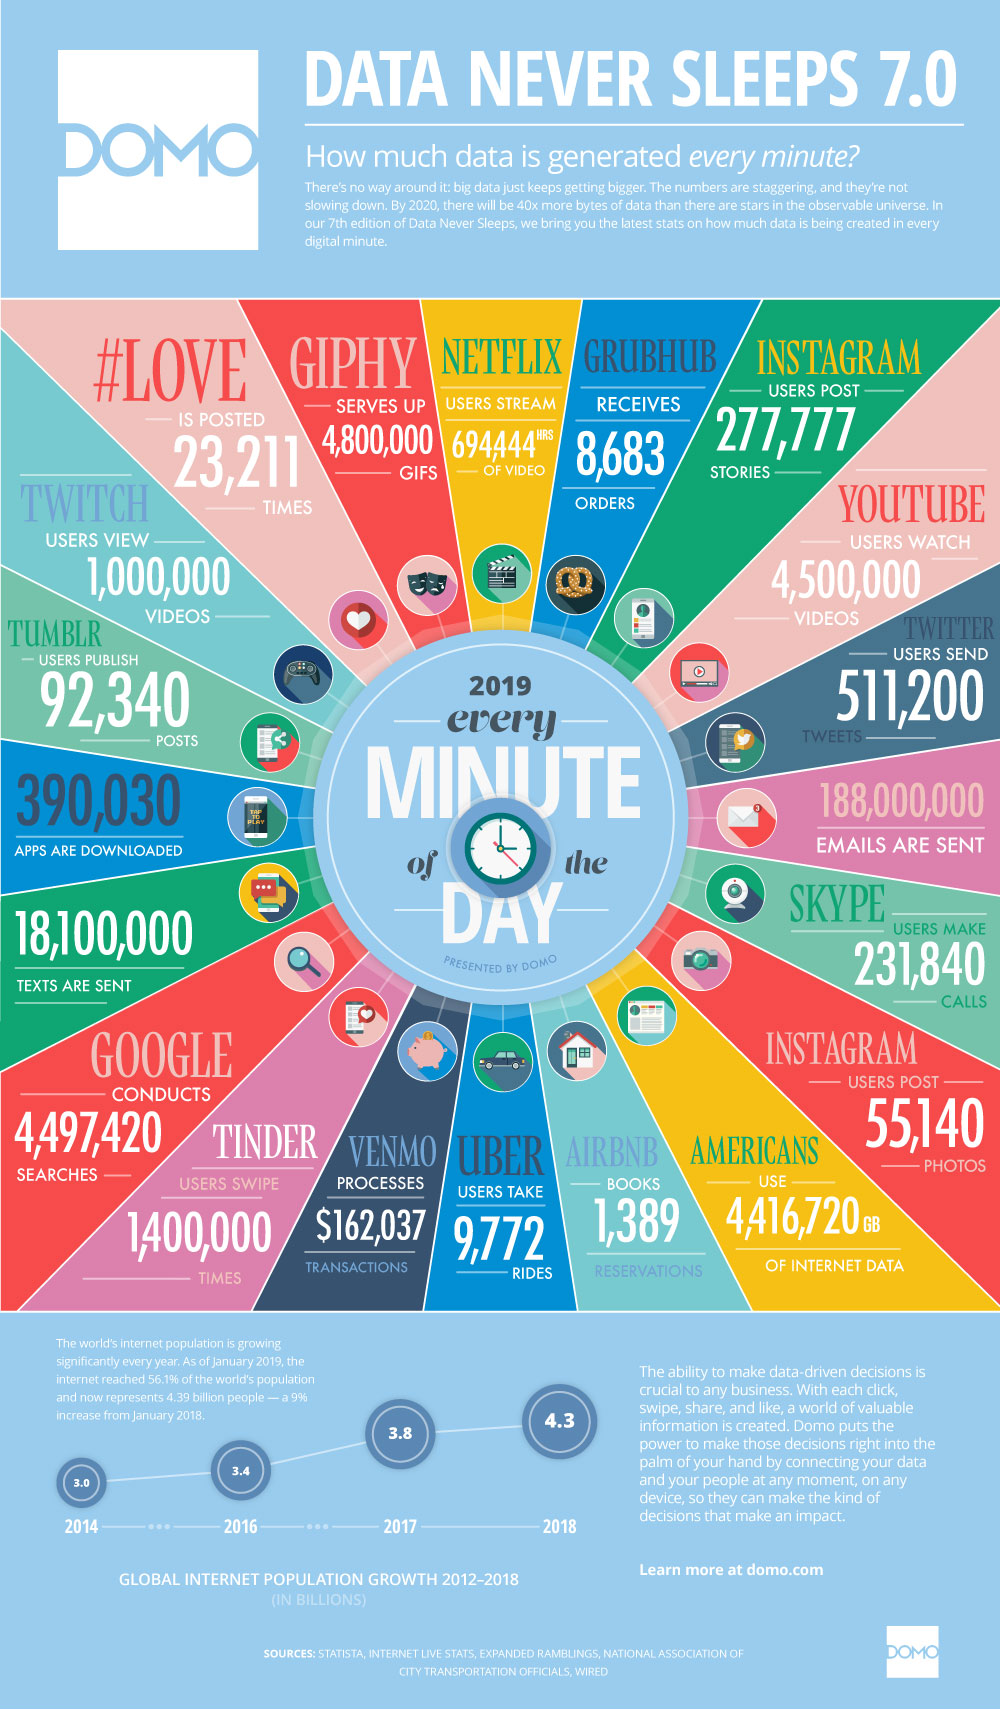
\includegraphics[width=\linewidth]{19_domo_data-never-sleeps-7}

Desde finales del sigo \textsc{xx} se ha considerado que vivimos en la ``era de la información", una etapa caracterizada por el incremento, desarrollo y propagación de emergentes tecnologías de la información y comunicación que han permitido al ser humano romper las barreras de la distancia, el tiempo y el lugar a la hora de comunicarse y compartir información; actividades que han sido decisivas en nuestra historia \cite{1}. Sin embargo, la era en la que realmente vivimos es la ``era de los datos", donde \textcolor{Red} {cada día se generan más de dos mil quinientos millones de petabytes\footnote {Un Petabyte es una unidad de información o almacienamiento de datos equivalente a un cuadrillon de bytes, mil terabytes o un millón de gigabytes. En este caso, es el equivalente a 2.5 quintillones de bytes.} de datos} provenientes de comercios, ciencias, Internet y casi cualquier actividad del día a día \cite{2} que acaban volcados en redes de ordenadores, sitios web, bases de datos y otros medios de almacenaje. 

Esta explosión de datos, a la que se ha denominado Big Data, se debe al alto grado de computarización de la sociedad y el avance de herramientas de recolección y almacenamiento de datos. Negocios en todo el mundo generan grandes cantidades de datos derivados de transacciones, stock de productos,  platillas de empleados, etc. Las ramas de la ciencia producen datos de manera constante frutos de experimentos, observaciones, recogida de muestras, etc. Y más recientemente, Internet y las redes sociales han sido las principales responsables del aumento excesivo de datos, siendo usadas por millones de personas simultáneamente.

Y, aunque esto ha supuesto una considerable mejora para la humanidad pues la información nunca había sido tan accesible, también ha traido consecuencias negativas y problemas como el almacenamiento y organización de los datos, datos no estructurados que entorpecen su acceso y procesamiento, dificultades a la hora de analizar los datos apropiadamente pudiendo generar desinformación y complicaciones para mostrar los resultados de forma apropiada y aplicarlos de manera eficiente y útil en el mundo real \cite{3}.

Como resultado, ha surgido una nueva ciencia que se ha posicionado rápidamente como una de las disciplinas más influyentes de la actualidad: Data Science (Ciencia de los Datos), que debido a su reciente aparición, carece de una definición consensuada, pero podríamos concretarla como ``\textit{Ciencia que usa Estadística, Inteligencia Artificial, Programación y Bases de Datos para posibilitar la extracción de conocimiento a partir de datos}" \cite{4}. A su vez, dentro de esta ciencia se han desarrollado otras tres ramas: Data Warehousing, Data Mining y Visualization; cada una de ellas enfocada a resolver o afrontar uno o varios de los problemas mencionados previamente: organización y agrupación de datos, análisis de los mismos y presentación de los resultados, respectivamente.

De entre estas nuevas disciplinas, Data Mining es la que se centra en el procesamiento de los datos, procedimiento por el cual se obtiene la información, y se podría definir como ''\textit{Proceso de descubrimiento de patrones interesantes y conocimiento a partir de grandes volúmenes de datos}" \cite{5}, donde dentro de la misma podemos encontrar diferentes técnicas para encontrar patrones y relaciones, y dependiendo de cuál se aplique se puede obtener un resultado totalmente diferente incluso con el mismo conjunto de datos, por lo que es fundamental emplear la técnica apropiada en función del del objetivo a conseguir, los datos con los que se pretende trabajar y el ámbito de aplicación.

Y en algunos de los campos más importantes del mundo moderno como la analítica de negocios, el reconocimiento de imágenes, las búsquedas web, seguridad, biología y ciencias de la salud; existen dificultades a la hora de clasificar o agrupar ciertos datos porque estos no disponen de una etiqueta o valor conocido por el que se pueda hacerlo, pues este no existe o no ha sido definido. Para poder afrontar este problema se utiliza la técnica de Clustering, que permite exactamente generar valores y etiquetas para un conjunto de datos realizando agrupaciones denominadas \textit{clusters} o grupos, donde los datos de un mismo cluster sean muy similares entre ellos y a su vez tengan diferencias claras con datos de otros clusters, permitiendo que cada grupo resultante puede ser etiquetado y tratado como una clase propia.

De esta manera, el objetivo de este Trabajo de Fin de Grado (TFG) es realizar un estudio sobre Clustering, exponiendo de manera teórica qué es este método y qué tipo de utilidades tiene, así como el desarrollo de las diferentes técnicas que existen y las aplicaciones que estas ofrecen. Posteriormente se explorará este método dentro de Bioinformática, un campo centrado en desarrollar técnicas y programas software para analizar datos biológicos, viendo qué aporta a dicha disciplina y cuáles de las técnicas expuestas previamente se emplean y por qué. 

Una vez realizado el marco teórico previo, se pretende hacer una parte práctica los diferentes paquetes que ofrecen técnicas de Clustering tanto de carácter general como dentro de Bioinformática para el lenguaje de programación R \cite{6}, uno de los más relevantes dentro de Data Science.


%====================================================================================================================================================%


\section{Clustering} 

Clustering o Cluster Analysis, adaptado al español como Clusterización, Agrupamiento o Análisis de Grupos, es un método de Data Mining que se basa en el Aprendizaje Automático (Machine Learning), una rama de la Inteligencia Artificial (Artificial Intelligence) que pretende desarrollar sistemas que resuelvan problemas basándose en los resultados de experiencias previas, aprendiendo de sus errores. Concretamente, se fundamenta en uno de los métodos de aprendizaje explorados en esta disciplina: Aprendizaje No Supervisado, enfocado en el desarrollo y descubrimiento de nuevos conocimientos. Este, a diferencia de otros métodos de aprendizaje, no dispone de conocimiento previo sobre lo que poder aprender, por lo que su objetivo principal es discernir patrones y relaciones entre los datos para poder separarlos \cite{7}.

En esencia, el proceso de Clustering es el mismo, hasta el punto en que básicamente podríamos considerarlos sinónimos, puesto que Clusterización se aplica principalmente sobre conjuntos de datos que se desean organizar en diferentes grupos pero los valores que delimitan cada cluster son desconocidos y por lo tanto se definen en el propio proceso de clasificación.

\textcolor{Red} {De una manera más técnica, podríamos decir que Clustering busca definir para una determinada característica\footnote{Dicho de una cualidad que da carácter o sirve para distinguir a algo o alguien de sus semejante.} o Suceso Elemental\footnote{Cada uno de los resultados más simples que se pueen obtener de la realización de un experimento. Obtener el número 3 al tirar un dado.} (SE), un conjunto de grupos de observaciones (suceso) \footnote{Se denomina así al subconjunto total de resultados posibles al realizar un experimento. Obtener un 3 o sacar par al tirar un dado.} con valores cercanos; donde los clusters permiten, dados los diferentes sucesos elementales que configuran un suceso, asignar cada SE al mismo cluster \cite{8}.}

Para poder decidir si dos datos deben ser agrupados en el mismo cluster o por el contrario, separados, es necesario introducir los conceptos de similaridad y disparidad; cuanto más similares sean los datos, más tendrán en común y por lo tanto es más probable que terminen bajo el mismo cluster, y por otra parte, si los datos son diferentes entre sí, serán separados en clusters diferentes. Este criterio se basa en la proximidad de dichos objetos. Si midiéramos la similitud entre dos objetos \textit{i} y \textit{j}, esta devolvería 0 si ambos fueran totalmente distintos, y cuanto más elevado fuera el valor, más semejantes serían, siendo 1 el valor más alto, indicando que ambos datos son idénticos. De la misma manera, medir la disparidad entre los objetos daría resultados opuestos, con un 0 indicando que son idénticos y con un 1 que no tienen nada en común. 

Esta forma de calcular la proximidad no solo ayuda a la hora de agrupar los datos en clusters y formar subconjuntos a partir de los resultados, sino que con este proceso también somos capaces de detectar outliers, datos anómalos que pueden ser datos erróneos procedentes de errores de medida o fallos que deben ser eliminados o, datos correctos sumamente importantes que son diferentes al esto y deben ser analizados detenidamente. A la hora de agrupar los datos, puede que queden varios objetos sueltos sin pertenecer a ningún cluster, esos son los datos anómalos.

Además, Clustering también sirve como primera aproximación a la hora de procesar los datos, porque aunque de por sí, este proceso puede aportar información útil agrupando datos similares y clasificándolos, permitiendo un análisis de los resultados que puede dar lugar al descubrimiento de nuevos conocimientos, también se usa como método de preprocesamiento de datos para otros algoritmos de Data Mining que trabajarán sobre las clusters generados y los atributos seleccionados como criterio a la hora de crearlos, pues estos se pueden considerar clases nuevas de objetos.

Es gracias a estas características que Clusterización es empleada en muchos ámbitos del mundo actual, siendo la técnica de Aprendizaje No Supervisado más extendida. Campos como la analítica de negocios, el reconocimiento de imágenes, las búsquedas web, seguridad, biología y ciencias de la salud hacen uso habitual de esta técnica para clasificar tipos de consumidores que comparten preferencias, aunar bajo un mismo subconjunto muchas formas diferentes de escribir el mismo caracter para facilitar el reconocimiento de textos escritos a mano, agrupar resultados similares de una consulta en internet y mostrar los más relevantes dentro de cada grupo o el estudio de la taxonomía\footnote{Ciencia que trata de los principios, métodos y fines de la clasificación. Se aplica en particular, dentro de la biología, para la ordenación jerarquizada y sistemática, con sus nombres, de los grupos de animales y de vegetales.} de las especies. También se puede hacer uso de su capacidad para detectar datos anómalos con la finalidad de revelar posibles fraudes o transacciones  financieras sospechosas, incluso ayudar en la disminución de crímenes analizando los resultados obtenidos tras clusterizar datos de detenciones y delitos; incluso aplicada a datos geofísicos\footnote{La Geofísica es la ciencia que estudia la Tierra desde el punto de vista de la física.} para interpretarlos y obtener resultados significativos. Asimismo, se utiliza a la hora de comparar comunidades en redes sociales permitiendo recomendar a los usuarios contenido de su agrado, o dentro del mundo sanitario, ayudando en la identificación y control de diversos tipos de enfermedades e incluso puede usarse como apoyo en la gestión de edificios públicos como bibliotecas, agrupando a los lectores por sus preferencias de manera similar a los consumidores de un negocio \cite{9,10,11,12,13}.

Agrupando toda esta información, podemos concretar los tres principales motivos por los que Clustering es empleado: clasificación natural, compresión y generación de una estructura base \cite{14}.

La utilidad de este método y la flexibilidad que ofrece con las diversas técnicas y formas de aplicarlo de las que dispone e es también parte fundamental de que sea tan comúnmente utilizado y con objetivos tan dispares en gran parte de las áreas del conocimiento. Sin embargo, también es un método frágil, pues depende en gran medida de los datos con los que se trabaje y el criterio escogido para determinar si dos objetos deben agruparse bajo el mismo cluster o separarlos, Por lo que es necesario seguir una serie de pasos a la hora de realizar un Análisis de Grupos de manera correcta \cite{15}:

\begin{enumerate}
\item Primero, hay que seleccionar cuidadosamente los datos con los que se va a trabajar, puesto que tanto el tipo de dato como la cantidad de los mismos influyen directamente en los resultados. Si se utilizan demasiados datos el procesamiento puede tener un coste computacional alto y es difícil ofrecer una visualización elegante de los resultados. Pero si se escogen pocos datos se pierde información útil y puede dar lugar a equivocaciones. Es por ello que este paso suele realizarlo un experto en el sector o con su ayuda. 
\item Segundo, se debe elegir la forma en la que se va a calcular la similaridad entre los diferentes datos, que analizaremos más adelante cuando analicemos las diferentes técnicas de Clustering.
\item Tercero, debe definirse el criterio con el que se va a tomar la decisión de agrupar en el mismo cluster dos datos. Es decir, escoger el umbral de similaridad a partir del cual dos datos pasan a formar parte del mismo cluster y qué característica o conjunto de ellas van a ser utilizadas para medir la similitud. La elección del umbral suele ser complicada, y es necesaria mucha experiencia o varias iteraciones de ensayo y error para encontrar un valor correcto.
\item Cuarto, hay que optar por uno de los diversos algoritmos de Clusterización que existen, pues los resultados pueden cambiar considerablemente al variar la estrategia con la que se realiza la agrupación. Estos se verán a continuación.
\item Por último, una vez obtenidos los resultados hay que validarlos e interpretarlos. La resolución de este paso depende del objetivo inicial por el que se haya decidido realizar el análisis.
\end{enumerate}

Como puede verse, tanto el paso inicial como el último requieren de la ayuda de personas cualificadas si pretenden realizarse correctamente, y es en los pasos intermedios donde la intervención de computadoras y programas informáticos son más útiles y están más desarrollados, pues permiten aligerar considerablemente la carga de trabajo y como consecuencia, se puede analizar una mayor cantidad de datos. Pero no deja de ser una tarea complicada que ha ocasionado una gran demanda de expertos en Data Mining y Data Science en diversas áreas de trabajo durante los últimos años.

La utilidad que aporta Clustering permitiendo crear grupos con datos similares entre sí y dispares con respecto a otros grupos con el fin de clasificarlos y las ventajas que esto presenta queda reflejada en la cantidad de usos que recibe, por lo que vamos a profundizar en las diferentes técnicas que son empleadas para la generación de los clusters y su funcionamiento que lo hacen tan importante.


%====================================================================================================================================================%
%====================================================================================================================================================%


\section{Técnicas de Clustering}

Existe una gran variedad de técnicas de Clustering que cumplen con el propósito de clasificar un conjunto de datos, pero no todas son iguales. Existen una serie de requisitos típicos que debe cumplir un algoritmo de Clusterización para satisfacer las expectativas y realizar un buen análisis. Sin embargo, cumplir todos estos requerimientos de forma simultánea es una tarea casi imposible, por lo que analizar cuáles ofrece cada algoritmo nos ayuda a identificar sus puntos fuertes y débiles y por ende, facilitar la elección del algoritmo apropiado para cada ocasión. Veamos cuáles son dichos requisitos y cómo podemos comparar algoritmos.

\subsection{\textbf{Requisitos de un algoritmo de Clustering}}

\cite{16} Sobre el papel, analizar datos no debería suponer un problema; pero la realidad es que existen trabas que complican este procedimiento tales como la cantidad de datos a analizar o el tipo de datos. Algunos de los algoritmos de Clustering iniciales no tenían en cuenta este tipo de problemas, porque no existían en su momento, pero ahora es necesario afrontarlos para que el análisis de los datos sea eficiente y produzca resultados completos y veraces.

A continuación, se exponen los requisitos típicos que se exigen dentro de Data Mining a un algoritmo de Clustering, así como debilidades que presentan algunos de los existentes.

\begin{itemize}
\item \textbf{Escalabilidad}: Muchos algoritmos de Clusterización trabajan bien con conjuntos de datos pequeños que contienen solo unos cuantos cientos de objetos; sin embargo, la gran mayoría de bases de datos contienen millones y miles de millones de datos. Analizar solo un pequeño porcentaje de esos datos puede resultar en conocimiento parcial, siendo necesario que sean escalables para resultados óptimos.

\item \textbf{Habilidad para lidiar con diferentes tipos de atributos}\footnote{Dicho de una característica cualitativa de un individuo o dato usada para distinguirlo de una variable o característica cuantitativa.}: Coloquialmente se suele entiende por atributo un dato\footnote{Valor obtenido para una característica en una observación.} cuantitativo, es decir, un número. Sin embargo, existen otros tipos de datos: nominales\footnote{Dicho de un dato cualitativo que proporciona suficiente información para nombrar a una característica y poder diferenciarla de otra.}, binarios\footnote{Datos que solo pueden tomar los valores cero y uno (0, 1).}, ordinales\footnote{Datos cualitativos que proporcionan suficiente información para ordenar las observaciones.}, imágenes, gráficos, documentos y mezclas de varios de estos tipos. Por lo que un algoritmo de Clustering debe estar preparado para lidiar con todos o la gran mayoría de ellos.

\item \textbf{Descubrimiento de clusters con formas arbitrarias}: Gran parte de los algoritmos utilizan formas de calcular la similaridad entre los datos basadas en la distancia entre los mismos, lo que suele dar lugar a clusters con formas redondas o esféricas. En determinadas ocasiones esto puede resultar contraproducente y erróneo, por lo que también es preciso que los algoritmos sean capaces de identificar diferentes formas de clusters, no solamente formas circulares o geométricas.

\item \textbf{Requirir información al usuario}: En algunos algoritmos de Clustering es común pedir cierto tipo de información al usuario a la hora de trabajar con los datos, como el número de clusters que se quieren generar. Este tipo de práctica puede ocasionar problemas dada la complejidad de esta decisión, sobre todo en escenarios en los que los datos cuentan con múltiples atributos. Por lo que es recomendable que los algoritmos eviten este comportamiento tanto para aliviar a los usuarios como para no comprometer la calidad a la hora de formar clusters, pues el algoritmo se adaptaría al valor introducido por el usuario, aunque fuese erróneo, generando también, un resultado errado.

\item \textbf{Capacidad para trabajar con ruido en los datos}: Aunque es común tratar de antemano los datos para eliminar cualquier tipo de dato no deseado, recordemos que esta técnica también se aplica como método de preprocesamiento para otros algoritmos de Data Mining, por lo que es necesario que no sean sensibles hacia estas impurezas, puesto que podría resultar en una clasificación pobre.

\item \textbf{Clusterización incremental e insensibilidad al orden de entrada}: Cuando se aplica Clustering en entornos en constante movimiento como el de los negocios, es común que se introduzcan datos nuevos junto a los ya existentes. Ciertos algoritmos no son compatibles con este incremento de información, y es necesario volver a iniciar un nuevo proceso de Clusterización. Mientras que otros que sí toleran este cambio, resulta que son sensibles respecto al orden con el que se han introducido los datos y pueden generar agrupaciones erróneas. Estos problemas han dado lugar a la necesidad de algoritmos que puedan lidiar con la incorporación de nuevos datos y que no se vean afectados por el orden en el que estos son introducidos.

\item \textbf{Capacidad de Clusterizar datos con muchos atributos}: Aunque de manera común se suele trabajar con datos que no contienen mucho más que una decena de atributos, hay ciertos tipos de datos como documentos, en los que cada palabra clave puede ser considerada un atributo, dando lugar a cientos de atributos por cada dato, haciendo complicado trabajar con ellos y también clasificarlos, por lo que se precisa de algoritmos que puedan lograr un buen resultado con este tipo de datos.

\item \textbf{Clustering basado en restricciones}: En el mundo real podemos encontrar ciertas barreras a la hora de aplicar un algoritmo de Clustering, en los que, por ejemplo, sí se tenga que tener en cuenta un límite a la cantidad de cluster que se pueden generar o de decidir si dos datos o clusters deban unirse. Aunque es complicado realizar este tipo de agrupaciones, es indispensable que los algoritmos obtengan resultados decentes dadas estas limitaciones.

\item \textbf{Interpretabilidad y usabilidad}: De nada sirve clasificar los datos y cumplir con los requisitos previos si no se puede interpretar el resultado. Los algoritmos, por lo tanto, deben ofrecer conclusiones comprensibles, coherentes y que puedan usarse, sometiéndose a ciertas limitaciones semánticas y visuales con la finalidad de acomodar el resultado al objetivo inicial por el que se ha llevado a cabo la clusterización.
\end{itemize}


%====================================================================================================================================================%


\subsection{\textbf{Criterios de comparación}}

\cite{16} Cada algoritmo opera de forma distinta en diferentes aspectos como el criterio de división, la separación de clusters, el cálculo de la similaridad y el espacio de clusterización. Observando los pasos a seguir y la toma de decisiones de un algoritmo, podemos compararlo con otro y escoger cuál es más adecuado para el problema a afrontar. 

\begin{itemize}
\item \textbf{Criterio de división}: Principalmente existen dos tipos de métodos respecto a este criterio, aquellos que fraccionan todos los datos para que no exista ningún tipo de orden o diferencia de nivel entre ellos, y los que, por el lado opuesto, dividen los datos de manera jerárquica, permitiendo formar clusters en diferentes niveles semánticos. Cada uno aporta una utilidad distinta, con el primer tipo de criterio podemos abordar problemas como la clasificación de clientes o lectores, conjuntos de datos en los todos reciben el mismo trato; mientras que con criterio de partición jerárquico podemos organizar documentos en varios campos como ``deportes", ``política" o ``comida", y dentro de cada campo tener subconjuntos como ``postres", ``pasta" o ``carne".

\item \textbf{Separación de clusters}: Otro criterio en el que hay dos enfoques: si un dato forma parte de un cluster, este no puede formar parte de otro a no ser que ambos clusters se unan; o permitir que un dato pueda estar en dos clusters a la vez, un concepto denominado ``Fuzzy clustering". La primera aproximación ofrece un enfoque más determinista que es quizás el más aplicado entre ambos métodos, pero existen disciplinas en las que permitir que un dato forme parte de más de cluster puede ser realmente útil y que cada vez recibe más usos \cite{17}.  

\item \textbf{Cálculo de similaridad}: Una de las pautas que más determina un algoritmo de clusterización es la forma en la que calculan la similaridad entre los datos, y que exploraremos detalladamente más adelante. Gran parte de los algoritmos utilizan la distancia que hay entre dos objetos para calcular su similaridad aplicando métodos como la distancia Euclídea o espacios vectoriales. Esta tipo de cálculo se ve beneficiado de métodos de optimización, pero suele generar clusters con formas esférica o cilíndricas, por lo que cada vez más se utilizan algoritmos que miden la similaridad entre objetos mediante la densidad o contigüidad del espacio para formar clusters, lo cual permite descubrir grupos con formas arbitrarias.  

\item \textbf{Espacio de Clusterización}: Muchos algoritmos de Clustering observan todo el espacio de datos para buscar grupos, que es un método totalmente factible y válido para datos con pocos atributos. Sin embargo, cuando se tratan de procesar datos con gran cantidad de atributos, es mejor centrarse en pequeñas partes del total, en subconjuntos de espacio y buscar clusters dentro de ellos de forma que se pueda obtener información valiosa a un menor coste computacional.
\end{itemize}


%====================================================================================================================================================%


\subsection{\textbf{Clasificación general de técnicas}}

\cite{16} Una vez que hemos visto los requisitos de los algoritmos de Clustering y los criterios para compararlos entre sí, podemos agrupar la mayor parte de las técnicas bajo cuatro grandes grupos que describiremos brevemente a continuación y sobre los que precisaremos individualmente en la siguiente sección, señalando los principales algoritmos dentro de cada una de ellos.

\begin{itemize}
\item \textbf{Métodos basados en particiones}:

\item \textbf{Métodos jerárquicos}:

\item \textbf{Métodos basados en densidad}:

\item \textbf{Métodos basados en cuadrícula o rejilla}:
\end{itemize}

%====================================================================================================================================================%
%====================================================================================================================================================%


\clearpage

\section{Referencias}
\renewcommand{\section}[2]{}
\begin{thebibliography}{X}

\bibitem{1} Alberts, D. S., \& Papp, D. S. (1997). \href{http://www.dodccrp.org/files/Alberts_Anthology_I.pdf} {The information age: An anthology on its impact and consequences}. Office of the Assistant Secretary of Defense Washington DC Command and Control Research Program (CCRP).

\bibitem{2} Becoming A Data-Driven CEO | Domo. (2018). Data never sleeps 6.0 \href{https://www.domo.com/solution/data-never-sleeps-6} {https://www.domo.com/solution/data-never-sleeps-6}

\bibitem{3} Xu, Z., \& Shi, Y. (2015). \href {https://link.springer.com/content/pdf/10.1007/s40745-015-0063-7.pdf} {Exploring big data analysis: fundamental scientific problems}´. Annals of Data Science, 2(4), 363-372.

\bibitem{4} Definición Data Science apuntes FCD

\bibitem{5} Definición Data Mining libro 100

\bibitem{6} The R Project for Statistical Computing. (n.d.). Retrieved from \href{https://www.r-project.org/} {https://www.r-project.org/}

\bibitem{7} Moreno, A. (1994). \href{https://upcommons.upc.edu/bitstream/handle/2099.3/36157/9788483019962.pdf?sequence=1&isAllowed=y} {Aprendizaje automático.} Llibre, Edicions UPC.

\bibitem{8} Apuntes JJ clustering

\bibitem{9} Alkhaibari, A. A., \& Chung, P. (2017). \href{https://ieeexplore.ieee.org/document/8001983} {Cluster analysis for reducing city crime rates}. 2017 IEEE Long Island Systems, Applications and Technology Conference (LISAT). doi:10.1109/lisat.2017.8001983

\bibitem{10} Song, Y., Meng, H., \& Zhang, Y. (2010). \href{https://ieeexplore.ieee.org/document/5602787} {Clustering analysis and its applications}. 2010 Second IITA International Conference on Geoscience and Remote Sensing. doi:10.1109/iita-grs.2010.5602787

\bibitem{11} Prabhu, J., Sudharshan, M., Saravanan, M., \& Prasad, G. (2010). \href{https://ieeexplore.ieee.org/document/5563072} {Augmenting Rapid Clustering Method for Social Network Analysis}. 2010 International Conference on Advances in Social Networks Analysis and Mining. doi:10.1109/asonam.2010.55

\bibitem{12} Baron, J. N., Aznar, M. N., Monterubbianesi, M., \& Martínez-López, B. (2020). \href{https://search.ebscohost.com/login.aspx?direct=true&db=aph&AN=143827917&lang=es&site=ehost-live&scope=site} {Application of network analysis and cluster analysis for better prevention and control of swine diseases in Argentina}. PLoS ONE, 15(6), 1–26. https://doi.org/10.1371/journal.pone.0234489

\bibitem{13} Li, J., \& Chen, P. (2008). \href{https://ieeexplore.ieee.org/document/4810639} {The application of Cluster analysis in Library system}. 2008 IEEE International Symposium on Knowledge Acquisition and Modeling Workshop. doi:10.1109/kamw.2008.4810639

\bibitem{14} Oyelade, J., Isewon, I., Oladipupo, O., Emebo, O., Omogbadegun, Z., Aromolaran, O., . . . Olawole, O. (2019). Data Clustering: Algorithms and Its Applications. 2019 19th International Conference on Computational Science and Its Applications (ICCSA). doi:10.1109/iccsa.2019.000-1

\bibitem{15} Carugo, O., \& Eisenhaber, F. (2010). Data Mining Techniques for the Life Sciences. Humana Press.
             
\bibitem{16}Han, J., Kamber, M., \& Pei, J. (2012). Data Mining: Concepts and Techniques (3rd ed., p.~740). 225 Wyman Street, Waltham, MA 02451, USA: Morgan Kaufmann Publishers, Elsevier.

\bibitem{17} Höppner, F., Klawonn, F., Kruse, R., \& Runkler, T. (1999). Fuzzy cluster analysis: methods for classification, data analysis and image recognition. John Wiley \& Sons.


\end{thebibliography}

\end{document}